\documentclass[a4paper,11pt,headings=standardclasses]{scrartcl}% see <http://www.komascript.de>
% ----------------------------------------------------------------------------
% font, style, etc.
\usepackage[utf8]{inputenc} % defines
\usepackage{csquotes}

% mathematics
\usepackage{amsmath}
\usepackage{amssymb}

% figures, tables, etc.
\usepackage{hyperref} %
\usepackage{graphicx}
\usepackage{tikz}
\usepackage{pgf}
\usepackage{xcolor}

% code
\usepackage{listings}
\lstset{
language=Python, 
backgroundcolor = \color{light-gray},
basicstyle=\scriptsize\sffamily,
stringstyle=\color{orange},
breaklines=true,
numberstyle=\tiny\color{gray},
keywordstyle=\bfseries\color{dark-blue}\textit, % print keywords dark-blue
commentstyle=\color{dark-green}, % print comments dark-green
showstringspaces=false} % spacing between strings not showed

% others
\usepackage{acronym}

% theorems
\newtheorem{defi}{Definition}[section]

% setup the appearance of links
\hypersetup{
    colorlinks = true, % false -> red box arround links (not very nice)
    linkcolor={red!20!black},
    citecolor={blue!50!black},
    urlcolor={blue!80!black},
}

% define shortcuts
\newcommand{\ad}{\mathrm{ad}}
\renewcommand{\d}{\mathrm{d}} % d vor differential forms
\newcommand{\NV}{{\cal N}\,}
\newcommand{\rang}{\mathrm{rang}}
\newcommand{\im}{\mathrm{im}}
\newcommand{\spann}{\mathrm{span}}
\newcommand{\R}{\mathbb{R}} %  set of real numbers
\newcommand{\py}{\emph{Python}\,}
\newcommand{\scipy}{\emph{SciPy}\,}
\newcommand{\mpl}{\emph{Matplotlib}\,}
\newcommand{\uu}{\mathbf{u}}
\newcommand{\x}{\mathbf{x}}
\newcommand{\y}{\mathbf{y}}
\newcommand{\z}{\mathbf{z}}
% color definitions
\definecolor{light-gray}{gray}{0.95}
\definecolor{dark-blue}{rgb}{0, 0, 0.5}
\definecolor{dark-red}{rgb}{0.5, 0, 0}
\definecolor{dark-green}{rgb}{0, 0.5, 0}
\definecolor{gray}{rgb}{0.5, 0.5, 0.5}

% ----------------------------------------------------------------------------
%\titlehead{Prof. Dr.-Ing. habli. Dipl.-Math. Klaus Röbenack \\ Institute of Control Theory \\ Faculty of Electrical and Computer Engineering \\TU Dresden, Germany}% optional
\subject{Control Theory Tutorial}% optional
\title{Car-Like Mobile Robot}
\subtitle{\py for simulation, animation and control}% optional
\author{}
\date{}
%\publishers{}% optional
% ----------------------------------------------------------------------------

\begin{document}
\maketitle% create title
\tableofcontents
\newpage
\section{Introduction}
The goal of this tutorial is to teach the usage of the programming language \py as a tool for developing and simulating control systems.

\section{Model of a car-like mobile robot}
\label{sec:model}
\begin{figure}[ht]
	\centering
	\def\svgwidth{0.7\textwidth}
	\input{img/car-like_mobile_robot.pdf_tex}
	\caption{Car-like mobile robot}
	\label{fig:car}
\end{figure}
Given is a nonlinear kinematic model of a car-like mobile robot, with the following system variables: position $(y_1, y_2)$ and orientation $\theta$ in the plane, the steering angle $\phi$ and the robots lateral velocity $v=\left| \mathbf{v} \right| $. 
\begin{subequations}\label{eq:syseq}
\begin{align}
\dot{y}_1&=v \cos (\theta) \\
\dot{y}_2&=v \sin (\theta) \\
\tan(\phi) &= \frac{l\dot{\theta}}{v}
\end{align}
\end{subequations}
To simulate this system of 1st order ordinary differential equations (ODEs), we define a state vector $\x=(x_1,x_2,x_3)^\mathrm{T}$ and a control vector $\uu=(u_1,u_2)^\mathrm{T}$:
\begin{align*}
x_1 &= y_1 & u_1 = v\\
x_2 &= y_2 & u_2 = \phi \\
x_3 &= \theta 
\end{align*}
Now we can express \eqref{eq:syseq} in a general form $\dot{\x}=f(\x,\uu)$:
\label{eq:ss_system}
\begin{align}
\underbrace{\begin{pmatrix} \dot{x}_1 \\ \dot{x}_2 \\ \dot{x}_3 \end{pmatrix}}_{\dot{\x}} = \underbrace{\begin{pmatrix}  u_1 \cos(x_3) \\ u_1 \sin(x_3) \\ \frac{1}{l}u_1 \tan(u_2) \end{pmatrix}}_{f(\x,\uu)}
\end{align}

\section{Storing parameters}
We store the parameters of our system in a class \emph{Parameters()}.
\begin{lstlisting}
class Parameters(object):
    pass
\end{lstlisting}
We therefore create an entity of \emph{Parameters()} and assign attributes.
\begin{lstlisting}
prmtrs = Parameters() # entity of class Parameters
prmtrs.l = 0.3 # define car length
prmtrs.w = prmtrs.l*0.3 # define car width
\end{lstlisting}

\section{Libraries and Packages}
In order to use $\cos(\cdot), \sin(\cdot)$ and $\tan(\cdot)$ we need to import these functions at the beginning of our code from the \emph{numpy} library.
\begin{lstlisting}
import numpy as np 
from numpy import cos, sin, tan
\end{lstlisting}
To simulate \eqref{eq:ss_system} we need to solve an initial value problem (IVP). In \py we can use the library \scipy and its sub-package \emph{integrate}, which delivers different solvers for IVPs.
\begin{lstlisting}
from scipy.integrate import odeint
\end{lstlisting}
For plotting the output of our simulation, we use the library \mpl and its sub-package \emph{pyplot}, which delivers a user experience similar to \emph{MATLAB}.
\begin{lstlisting}
import matplotlib.pyplot as plt
\end{lstlisting}
\section{Simulation with SciPy's integrate package}
\label{sec:simulation}
\footnote{corresponding file: \emph{car-like\_mobile\_robot\_plotting.py}}
To simulate \eqref{eq:ss_system} we need to implement the ODE system as a function in \py.
\lstinputlisting[numbers=left,firstnumber=7,firstline=7,lastline=26]{../sim/car-like_mobile_robot_plotting.py}
The control law is also implemented as function.
\lstinputlisting[numbers=left,firstnumber=29,firstline=29,lastline=41]{../sim/car-like_mobile_robot_plotting.py}
As a first simple heuristic, we set $(u_1, u_2)$ equal to constant values. Later we can implement an arbitrary function, for expample a feedback law $\uu=k(\x)$.

\subsection{Solution of the initial value problem (IVP) using \scipy}
We then define the simulation time and the initial state value.
\lstinputlisting[numbers=left,firstnumber=98,firstline=98,lastline=106]{../sim/car-like_mobile_robot_plotting.py}
Now we can parse these parameters and our ODE function to the solver.
\lstinputlisting[numbers=left,firstnumber=108,firstline=108,lastline=110]{../sim/car-like_mobile_robot_plotting.py}
The output is an array of size length(tt)$\times$length($\x$).

\section{Plotting using \mpl}
\label{sec:plot}
We encase our plotting instructions in a function. This way, we can define parameters of our plot, which we would like to change easily, for example figure width, or if the figure should be saved on the hard drive.
% def plot_data():
\lstinputlisting[numbers=left,firstnumber=44,firstline=44,lastline=91]{../sim/car-like_mobile_robot_plotting.py}
Now that we have defined our plotting function, we  can execute it with the calculated trajectories and our desired values for the functions parameters.
\lstinputlisting[numbers=left,firstnumber=115,firstline=115,lastline=118]{../sim/car-like_mobile_robot_plotting.py}
If your not satisfied with the result, you can change other properties of the plot, like linewidth or -color and many others easily. Just look up the documentation of \mpl : \url{https://matplotlib.org/index.html}
\begin{figure}[h]
\label{fig:state_traj}
   \centering      
   %% Creator: Matplotlib, PGF backend
%%
%% To include the figure in your LaTeX document, write
%%   \input{<filename>.pgf}
%%
%% Make sure the required packages are loaded in your preamble
%%   \usepackage{pgf}
%%
%% Figures using additional raster images can only be included by \input if
%% they are in the same directory as the main LaTeX file. For loading figures
%% from other directories you can use the `import` package
%%   \usepackage{import}
%% and then include the figures with
%%   \import{<path to file>}{<filename>.pgf}
%%
%% Matplotlib used the following preamble
%%   \usepackage{fontspec}
%%   \setmainfont{Times New Roman}
%%   \setsansfont{Lucida Grande}
%%   \setmonofont{Andale Mono}
%%
\begingroup%
\makeatletter%
\begin{pgfpicture}%
\pgfpathrectangle{\pgfpointorigin}{\pgfqpoint{4.724409in}{3.149606in}}%
\pgfusepath{use as bounding box, clip}%
\begin{pgfscope}%
\pgfsetbuttcap%
\pgfsetmiterjoin%
\definecolor{currentfill}{rgb}{1.000000,1.000000,1.000000}%
\pgfsetfillcolor{currentfill}%
\pgfsetlinewidth{0.000000pt}%
\definecolor{currentstroke}{rgb}{1.000000,1.000000,1.000000}%
\pgfsetstrokecolor{currentstroke}%
\pgfsetdash{}{0pt}%
\pgfpathmoveto{\pgfqpoint{0.000000in}{0.000000in}}%
\pgfpathlineto{\pgfqpoint{4.724409in}{0.000000in}}%
\pgfpathlineto{\pgfqpoint{4.724409in}{3.149606in}}%
\pgfpathlineto{\pgfqpoint{0.000000in}{3.149606in}}%
\pgfpathclose%
\pgfusepath{fill}%
\end{pgfscope}%
\begin{pgfscope}%
\pgfsetbuttcap%
\pgfsetmiterjoin%
\definecolor{currentfill}{rgb}{1.000000,1.000000,1.000000}%
\pgfsetfillcolor{currentfill}%
\pgfsetlinewidth{0.000000pt}%
\definecolor{currentstroke}{rgb}{0.000000,0.000000,0.000000}%
\pgfsetstrokecolor{currentstroke}%
\pgfsetstrokeopacity{0.000000}%
\pgfsetdash{}{0pt}%
\pgfpathmoveto{\pgfqpoint{0.530278in}{1.963970in}}%
\pgfpathlineto{\pgfqpoint{4.539409in}{1.963970in}}%
\pgfpathlineto{\pgfqpoint{4.539409in}{2.964606in}}%
\pgfpathlineto{\pgfqpoint{0.530278in}{2.964606in}}%
\pgfpathclose%
\pgfusepath{fill}%
\end{pgfscope}%
\begin{pgfscope}%
\pgfpathrectangle{\pgfqpoint{0.530278in}{1.963970in}}{\pgfqpoint{4.009132in}{1.000636in}} %
\pgfusepath{clip}%
\pgfsetrectcap%
\pgfsetroundjoin%
\pgfsetlinewidth{0.803000pt}%
\definecolor{currentstroke}{rgb}{0.690196,0.690196,0.690196}%
\pgfsetstrokecolor{currentstroke}%
\pgfsetdash{}{0pt}%
\pgfpathmoveto{\pgfqpoint{0.712511in}{1.963970in}}%
\pgfpathlineto{\pgfqpoint{0.712511in}{2.964606in}}%
\pgfusepath{stroke}%
\end{pgfscope}%
\begin{pgfscope}%
\pgfsetbuttcap%
\pgfsetroundjoin%
\definecolor{currentfill}{rgb}{0.000000,0.000000,0.000000}%
\pgfsetfillcolor{currentfill}%
\pgfsetlinewidth{0.803000pt}%
\definecolor{currentstroke}{rgb}{0.000000,0.000000,0.000000}%
\pgfsetstrokecolor{currentstroke}%
\pgfsetdash{}{0pt}%
\pgfsys@defobject{currentmarker}{\pgfqpoint{0.000000in}{-0.048611in}}{\pgfqpoint{0.000000in}{0.000000in}}{%
\pgfpathmoveto{\pgfqpoint{0.000000in}{0.000000in}}%
\pgfpathlineto{\pgfqpoint{0.000000in}{-0.048611in}}%
\pgfusepath{stroke,fill}%
}%
\begin{pgfscope}%
\pgfsys@transformshift{0.712511in}{1.963970in}%
\pgfsys@useobject{currentmarker}{}%
\end{pgfscope}%
\end{pgfscope}%
\begin{pgfscope}%
\pgfpathrectangle{\pgfqpoint{0.530278in}{1.963970in}}{\pgfqpoint{4.009132in}{1.000636in}} %
\pgfusepath{clip}%
\pgfsetrectcap%
\pgfsetroundjoin%
\pgfsetlinewidth{0.803000pt}%
\definecolor{currentstroke}{rgb}{0.690196,0.690196,0.690196}%
\pgfsetstrokecolor{currentstroke}%
\pgfsetdash{}{0pt}%
\pgfpathmoveto{\pgfqpoint{1.444372in}{1.963970in}}%
\pgfpathlineto{\pgfqpoint{1.444372in}{2.964606in}}%
\pgfusepath{stroke}%
\end{pgfscope}%
\begin{pgfscope}%
\pgfsetbuttcap%
\pgfsetroundjoin%
\definecolor{currentfill}{rgb}{0.000000,0.000000,0.000000}%
\pgfsetfillcolor{currentfill}%
\pgfsetlinewidth{0.803000pt}%
\definecolor{currentstroke}{rgb}{0.000000,0.000000,0.000000}%
\pgfsetstrokecolor{currentstroke}%
\pgfsetdash{}{0pt}%
\pgfsys@defobject{currentmarker}{\pgfqpoint{0.000000in}{-0.048611in}}{\pgfqpoint{0.000000in}{0.000000in}}{%
\pgfpathmoveto{\pgfqpoint{0.000000in}{0.000000in}}%
\pgfpathlineto{\pgfqpoint{0.000000in}{-0.048611in}}%
\pgfusepath{stroke,fill}%
}%
\begin{pgfscope}%
\pgfsys@transformshift{1.444372in}{1.963970in}%
\pgfsys@useobject{currentmarker}{}%
\end{pgfscope}%
\end{pgfscope}%
\begin{pgfscope}%
\pgfpathrectangle{\pgfqpoint{0.530278in}{1.963970in}}{\pgfqpoint{4.009132in}{1.000636in}} %
\pgfusepath{clip}%
\pgfsetrectcap%
\pgfsetroundjoin%
\pgfsetlinewidth{0.803000pt}%
\definecolor{currentstroke}{rgb}{0.690196,0.690196,0.690196}%
\pgfsetstrokecolor{currentstroke}%
\pgfsetdash{}{0pt}%
\pgfpathmoveto{\pgfqpoint{2.176232in}{1.963970in}}%
\pgfpathlineto{\pgfqpoint{2.176232in}{2.964606in}}%
\pgfusepath{stroke}%
\end{pgfscope}%
\begin{pgfscope}%
\pgfsetbuttcap%
\pgfsetroundjoin%
\definecolor{currentfill}{rgb}{0.000000,0.000000,0.000000}%
\pgfsetfillcolor{currentfill}%
\pgfsetlinewidth{0.803000pt}%
\definecolor{currentstroke}{rgb}{0.000000,0.000000,0.000000}%
\pgfsetstrokecolor{currentstroke}%
\pgfsetdash{}{0pt}%
\pgfsys@defobject{currentmarker}{\pgfqpoint{0.000000in}{-0.048611in}}{\pgfqpoint{0.000000in}{0.000000in}}{%
\pgfpathmoveto{\pgfqpoint{0.000000in}{0.000000in}}%
\pgfpathlineto{\pgfqpoint{0.000000in}{-0.048611in}}%
\pgfusepath{stroke,fill}%
}%
\begin{pgfscope}%
\pgfsys@transformshift{2.176232in}{1.963970in}%
\pgfsys@useobject{currentmarker}{}%
\end{pgfscope}%
\end{pgfscope}%
\begin{pgfscope}%
\pgfpathrectangle{\pgfqpoint{0.530278in}{1.963970in}}{\pgfqpoint{4.009132in}{1.000636in}} %
\pgfusepath{clip}%
\pgfsetrectcap%
\pgfsetroundjoin%
\pgfsetlinewidth{0.803000pt}%
\definecolor{currentstroke}{rgb}{0.690196,0.690196,0.690196}%
\pgfsetstrokecolor{currentstroke}%
\pgfsetdash{}{0pt}%
\pgfpathmoveto{\pgfqpoint{2.908092in}{1.963970in}}%
\pgfpathlineto{\pgfqpoint{2.908092in}{2.964606in}}%
\pgfusepath{stroke}%
\end{pgfscope}%
\begin{pgfscope}%
\pgfsetbuttcap%
\pgfsetroundjoin%
\definecolor{currentfill}{rgb}{0.000000,0.000000,0.000000}%
\pgfsetfillcolor{currentfill}%
\pgfsetlinewidth{0.803000pt}%
\definecolor{currentstroke}{rgb}{0.000000,0.000000,0.000000}%
\pgfsetstrokecolor{currentstroke}%
\pgfsetdash{}{0pt}%
\pgfsys@defobject{currentmarker}{\pgfqpoint{0.000000in}{-0.048611in}}{\pgfqpoint{0.000000in}{0.000000in}}{%
\pgfpathmoveto{\pgfqpoint{0.000000in}{0.000000in}}%
\pgfpathlineto{\pgfqpoint{0.000000in}{-0.048611in}}%
\pgfusepath{stroke,fill}%
}%
\begin{pgfscope}%
\pgfsys@transformshift{2.908092in}{1.963970in}%
\pgfsys@useobject{currentmarker}{}%
\end{pgfscope}%
\end{pgfscope}%
\begin{pgfscope}%
\pgfpathrectangle{\pgfqpoint{0.530278in}{1.963970in}}{\pgfqpoint{4.009132in}{1.000636in}} %
\pgfusepath{clip}%
\pgfsetrectcap%
\pgfsetroundjoin%
\pgfsetlinewidth{0.803000pt}%
\definecolor{currentstroke}{rgb}{0.690196,0.690196,0.690196}%
\pgfsetstrokecolor{currentstroke}%
\pgfsetdash{}{0pt}%
\pgfpathmoveto{\pgfqpoint{3.639953in}{1.963970in}}%
\pgfpathlineto{\pgfqpoint{3.639953in}{2.964606in}}%
\pgfusepath{stroke}%
\end{pgfscope}%
\begin{pgfscope}%
\pgfsetbuttcap%
\pgfsetroundjoin%
\definecolor{currentfill}{rgb}{0.000000,0.000000,0.000000}%
\pgfsetfillcolor{currentfill}%
\pgfsetlinewidth{0.803000pt}%
\definecolor{currentstroke}{rgb}{0.000000,0.000000,0.000000}%
\pgfsetstrokecolor{currentstroke}%
\pgfsetdash{}{0pt}%
\pgfsys@defobject{currentmarker}{\pgfqpoint{0.000000in}{-0.048611in}}{\pgfqpoint{0.000000in}{0.000000in}}{%
\pgfpathmoveto{\pgfqpoint{0.000000in}{0.000000in}}%
\pgfpathlineto{\pgfqpoint{0.000000in}{-0.048611in}}%
\pgfusepath{stroke,fill}%
}%
\begin{pgfscope}%
\pgfsys@transformshift{3.639953in}{1.963970in}%
\pgfsys@useobject{currentmarker}{}%
\end{pgfscope}%
\end{pgfscope}%
\begin{pgfscope}%
\pgfpathrectangle{\pgfqpoint{0.530278in}{1.963970in}}{\pgfqpoint{4.009132in}{1.000636in}} %
\pgfusepath{clip}%
\pgfsetrectcap%
\pgfsetroundjoin%
\pgfsetlinewidth{0.803000pt}%
\definecolor{currentstroke}{rgb}{0.690196,0.690196,0.690196}%
\pgfsetstrokecolor{currentstroke}%
\pgfsetdash{}{0pt}%
\pgfpathmoveto{\pgfqpoint{4.371813in}{1.963970in}}%
\pgfpathlineto{\pgfqpoint{4.371813in}{2.964606in}}%
\pgfusepath{stroke}%
\end{pgfscope}%
\begin{pgfscope}%
\pgfsetbuttcap%
\pgfsetroundjoin%
\definecolor{currentfill}{rgb}{0.000000,0.000000,0.000000}%
\pgfsetfillcolor{currentfill}%
\pgfsetlinewidth{0.803000pt}%
\definecolor{currentstroke}{rgb}{0.000000,0.000000,0.000000}%
\pgfsetstrokecolor{currentstroke}%
\pgfsetdash{}{0pt}%
\pgfsys@defobject{currentmarker}{\pgfqpoint{0.000000in}{-0.048611in}}{\pgfqpoint{0.000000in}{0.000000in}}{%
\pgfpathmoveto{\pgfqpoint{0.000000in}{0.000000in}}%
\pgfpathlineto{\pgfqpoint{0.000000in}{-0.048611in}}%
\pgfusepath{stroke,fill}%
}%
\begin{pgfscope}%
\pgfsys@transformshift{4.371813in}{1.963970in}%
\pgfsys@useobject{currentmarker}{}%
\end{pgfscope}%
\end{pgfscope}%
\begin{pgfscope}%
\pgftext[x=2.534844in,y=1.908414in,,top]{\sffamily\fontsize{10.000000}{12.000000}\selectfont t in s}%
\end{pgfscope}%
\begin{pgfscope}%
\pgfpathrectangle{\pgfqpoint{0.530278in}{1.963970in}}{\pgfqpoint{4.009132in}{1.000636in}} %
\pgfusepath{clip}%
\pgfsetrectcap%
\pgfsetroundjoin%
\pgfsetlinewidth{0.803000pt}%
\definecolor{currentstroke}{rgb}{0.690196,0.690196,0.690196}%
\pgfsetstrokecolor{currentstroke}%
\pgfsetdash{}{0pt}%
\pgfpathmoveto{\pgfqpoint{0.530278in}{2.312661in}}%
\pgfpathlineto{\pgfqpoint{4.539409in}{2.312661in}}%
\pgfusepath{stroke}%
\end{pgfscope}%
\begin{pgfscope}%
\pgfsetbuttcap%
\pgfsetroundjoin%
\definecolor{currentfill}{rgb}{0.000000,0.000000,0.000000}%
\pgfsetfillcolor{currentfill}%
\pgfsetlinewidth{0.803000pt}%
\definecolor{currentstroke}{rgb}{0.000000,0.000000,0.000000}%
\pgfsetstrokecolor{currentstroke}%
\pgfsetdash{}{0pt}%
\pgfsys@defobject{currentmarker}{\pgfqpoint{-0.048611in}{0.000000in}}{\pgfqpoint{0.000000in}{0.000000in}}{%
\pgfpathmoveto{\pgfqpoint{0.000000in}{0.000000in}}%
\pgfpathlineto{\pgfqpoint{-0.048611in}{0.000000in}}%
\pgfusepath{stroke,fill}%
}%
\begin{pgfscope}%
\pgfsys@transformshift{0.530278in}{2.312661in}%
\pgfsys@useobject{currentmarker}{}%
\end{pgfscope}%
\end{pgfscope}%
\begin{pgfscope}%
\pgftext[x=0.345233in,y=2.259119in,left,base]{\sffamily\fontsize{10.000000}{12.000000}\selectfont 0}%
\end{pgfscope}%
\begin{pgfscope}%
\pgfpathrectangle{\pgfqpoint{0.530278in}{1.963970in}}{\pgfqpoint{4.009132in}{1.000636in}} %
\pgfusepath{clip}%
\pgfsetrectcap%
\pgfsetroundjoin%
\pgfsetlinewidth{0.803000pt}%
\definecolor{currentstroke}{rgb}{0.690196,0.690196,0.690196}%
\pgfsetstrokecolor{currentstroke}%
\pgfsetdash{}{0pt}%
\pgfpathmoveto{\pgfqpoint{0.530278in}{2.828856in}}%
\pgfpathlineto{\pgfqpoint{4.539409in}{2.828856in}}%
\pgfusepath{stroke}%
\end{pgfscope}%
\begin{pgfscope}%
\pgfsetbuttcap%
\pgfsetroundjoin%
\definecolor{currentfill}{rgb}{0.000000,0.000000,0.000000}%
\pgfsetfillcolor{currentfill}%
\pgfsetlinewidth{0.803000pt}%
\definecolor{currentstroke}{rgb}{0.000000,0.000000,0.000000}%
\pgfsetstrokecolor{currentstroke}%
\pgfsetdash{}{0pt}%
\pgfsys@defobject{currentmarker}{\pgfqpoint{-0.048611in}{0.000000in}}{\pgfqpoint{0.000000in}{0.000000in}}{%
\pgfpathmoveto{\pgfqpoint{0.000000in}{0.000000in}}%
\pgfpathlineto{\pgfqpoint{-0.048611in}{0.000000in}}%
\pgfusepath{stroke,fill}%
}%
\begin{pgfscope}%
\pgfsys@transformshift{0.530278in}{2.828856in}%
\pgfsys@useobject{currentmarker}{}%
\end{pgfscope}%
\end{pgfscope}%
\begin{pgfscope}%
\pgftext[x=0.345233in,y=2.775315in,left,base]{\sffamily\fontsize{10.000000}{12.000000}\selectfont 2}%
\end{pgfscope}%
\begin{pgfscope}%
\pgftext[x=0.289677in,y=2.464288in,,bottom,rotate=90.000000]{\sffamily\fontsize{10.000000}{12.000000}\selectfont m}%
\end{pgfscope}%
\begin{pgfscope}%
\pgfpathrectangle{\pgfqpoint{0.530278in}{1.963970in}}{\pgfqpoint{4.009132in}{1.000636in}} %
\pgfusepath{clip}%
\pgfsetrectcap%
\pgfsetroundjoin%
\pgfsetlinewidth{1.003750pt}%
\definecolor{currentstroke}{rgb}{1.000000,0.000000,0.000000}%
\pgfsetstrokecolor{currentstroke}%
\pgfsetdash{}{0pt}%
\pgfpathmoveto{\pgfqpoint{0.712511in}{2.312661in}}%
\pgfpathlineto{\pgfqpoint{0.829609in}{2.394235in}}%
\pgfpathlineto{\pgfqpoint{0.902795in}{2.442533in}}%
\pgfpathlineto{\pgfqpoint{0.961344in}{2.478532in}}%
\pgfpathlineto{\pgfqpoint{1.019892in}{2.511459in}}%
\pgfpathlineto{\pgfqpoint{1.063804in}{2.533770in}}%
\pgfpathlineto{\pgfqpoint{1.107716in}{2.553776in}}%
\pgfpathlineto{\pgfqpoint{1.151627in}{2.571269in}}%
\pgfpathlineto{\pgfqpoint{1.195539in}{2.586067in}}%
\pgfpathlineto{\pgfqpoint{1.239451in}{2.598014in}}%
\pgfpathlineto{\pgfqpoint{1.283362in}{2.606988in}}%
\pgfpathlineto{\pgfqpoint{1.327274in}{2.612894in}}%
\pgfpathlineto{\pgfqpoint{1.371185in}{2.615671in}}%
\pgfpathlineto{\pgfqpoint{1.415097in}{2.615289in}}%
\pgfpathlineto{\pgfqpoint{1.459009in}{2.611754in}}%
\pgfpathlineto{\pgfqpoint{1.502920in}{2.605101in}}%
\pgfpathlineto{\pgfqpoint{1.546832in}{2.595399in}}%
\pgfpathlineto{\pgfqpoint{1.590744in}{2.582751in}}%
\pgfpathlineto{\pgfqpoint{1.634655in}{2.567288in}}%
\pgfpathlineto{\pgfqpoint{1.678567in}{2.549171in}}%
\pgfpathlineto{\pgfqpoint{1.722478in}{2.528588in}}%
\pgfpathlineto{\pgfqpoint{1.766390in}{2.505755in}}%
\pgfpathlineto{\pgfqpoint{1.824939in}{2.472225in}}%
\pgfpathlineto{\pgfqpoint{1.883488in}{2.435740in}}%
\pgfpathlineto{\pgfqpoint{1.956674in}{2.387012in}}%
\pgfpathlineto{\pgfqpoint{2.059134in}{2.315511in}}%
\pgfpathlineto{\pgfqpoint{2.190869in}{2.223914in}}%
\pgfpathlineto{\pgfqpoint{2.264055in}{2.176075in}}%
\pgfpathlineto{\pgfqpoint{2.322604in}{2.140584in}}%
\pgfpathlineto{\pgfqpoint{2.366516in}{2.116024in}}%
\pgfpathlineto{\pgfqpoint{2.410427in}{2.093512in}}%
\pgfpathlineto{\pgfqpoint{2.454339in}{2.073285in}}%
\pgfpathlineto{\pgfqpoint{2.498251in}{2.055552in}}%
\pgfpathlineto{\pgfqpoint{2.542162in}{2.040500in}}%
\pgfpathlineto{\pgfqpoint{2.586074in}{2.028284in}}%
\pgfpathlineto{\pgfqpoint{2.629985in}{2.019032in}}%
\pgfpathlineto{\pgfqpoint{2.673897in}{2.012841in}}%
\pgfpathlineto{\pgfqpoint{2.717809in}{2.009775in}}%
\pgfpathlineto{\pgfqpoint{2.761720in}{2.009865in}}%
\pgfpathlineto{\pgfqpoint{2.805632in}{2.013112in}}%
\pgfpathlineto{\pgfqpoint{2.849544in}{2.019480in}}%
\pgfpathlineto{\pgfqpoint{2.893455in}{2.028905in}}%
\pgfpathlineto{\pgfqpoint{2.937367in}{2.041287in}}%
\pgfpathlineto{\pgfqpoint{2.981279in}{2.056497in}}%
\pgfpathlineto{\pgfqpoint{3.025190in}{2.074378in}}%
\pgfpathlineto{\pgfqpoint{3.069102in}{2.094742in}}%
\pgfpathlineto{\pgfqpoint{3.113013in}{2.117377in}}%
\pgfpathlineto{\pgfqpoint{3.171562in}{2.150680in}}%
\pgfpathlineto{\pgfqpoint{3.230111in}{2.186982in}}%
\pgfpathlineto{\pgfqpoint{3.303297in}{2.235550in}}%
\pgfpathlineto{\pgfqpoint{3.405758in}{2.306961in}}%
\pgfpathlineto{\pgfqpoint{3.537492in}{2.398679in}}%
\pgfpathlineto{\pgfqpoint{3.610679in}{2.446696in}}%
\pgfpathlineto{\pgfqpoint{3.669227in}{2.482383in}}%
\pgfpathlineto{\pgfqpoint{3.727776in}{2.514927in}}%
\pgfpathlineto{\pgfqpoint{3.771688in}{2.536908in}}%
\pgfpathlineto{\pgfqpoint{3.815599in}{2.556552in}}%
\pgfpathlineto{\pgfqpoint{3.859511in}{2.573653in}}%
\pgfpathlineto{\pgfqpoint{3.903423in}{2.588035in}}%
\pgfpathlineto{\pgfqpoint{3.947334in}{2.599546in}}%
\pgfpathlineto{\pgfqpoint{3.991246in}{2.608067in}}%
\pgfpathlineto{\pgfqpoint{4.035158in}{2.613509in}}%
\pgfpathlineto{\pgfqpoint{4.079069in}{2.615815in}}%
\pgfpathlineto{\pgfqpoint{4.122981in}{2.614961in}}%
\pgfpathlineto{\pgfqpoint{4.166892in}{2.610957in}}%
\pgfpathlineto{\pgfqpoint{4.210804in}{2.603844in}}%
\pgfpathlineto{\pgfqpoint{4.254716in}{2.593695in}}%
\pgfpathlineto{\pgfqpoint{4.298627in}{2.580618in}}%
\pgfpathlineto{\pgfqpoint{4.342539in}{2.564747in}}%
\pgfpathlineto{\pgfqpoint{4.357176in}{2.558864in}}%
\pgfpathlineto{\pgfqpoint{4.357176in}{2.558864in}}%
\pgfusepath{stroke}%
\end{pgfscope}%
\begin{pgfscope}%
\pgfpathrectangle{\pgfqpoint{0.530278in}{1.963970in}}{\pgfqpoint{4.009132in}{1.000636in}} %
\pgfusepath{clip}%
\pgfsetrectcap%
\pgfsetroundjoin%
\pgfsetlinewidth{1.003750pt}%
\definecolor{currentstroke}{rgb}{0.000000,0.000000,1.000000}%
\pgfsetstrokecolor{currentstroke}%
\pgfsetdash{}{0pt}%
\pgfpathmoveto{\pgfqpoint{0.712511in}{2.312661in}}%
\pgfpathlineto{\pgfqpoint{0.756423in}{2.314241in}}%
\pgfpathlineto{\pgfqpoint{0.800334in}{2.318966in}}%
\pgfpathlineto{\pgfqpoint{0.844246in}{2.326785in}}%
\pgfpathlineto{\pgfqpoint{0.888158in}{2.337618in}}%
\pgfpathlineto{\pgfqpoint{0.932069in}{2.351351in}}%
\pgfpathlineto{\pgfqpoint{0.975981in}{2.367841in}}%
\pgfpathlineto{\pgfqpoint{1.019892in}{2.386917in}}%
\pgfpathlineto{\pgfqpoint{1.063804in}{2.408380in}}%
\pgfpathlineto{\pgfqpoint{1.107716in}{2.432006in}}%
\pgfpathlineto{\pgfqpoint{1.166265in}{2.466442in}}%
\pgfpathlineto{\pgfqpoint{1.224813in}{2.503647in}}%
\pgfpathlineto{\pgfqpoint{1.297999in}{2.552990in}}%
\pgfpathlineto{\pgfqpoint{1.444372in}{2.655654in}}%
\pgfpathlineto{\pgfqpoint{1.532195in}{2.715810in}}%
\pgfpathlineto{\pgfqpoint{1.590744in}{2.753755in}}%
\pgfpathlineto{\pgfqpoint{1.649292in}{2.789146in}}%
\pgfpathlineto{\pgfqpoint{1.693204in}{2.813618in}}%
\pgfpathlineto{\pgfqpoint{1.737116in}{2.836030in}}%
\pgfpathlineto{\pgfqpoint{1.781027in}{2.856147in}}%
\pgfpathlineto{\pgfqpoint{1.824939in}{2.873760in}}%
\pgfpathlineto{\pgfqpoint{1.868851in}{2.888685in}}%
\pgfpathlineto{\pgfqpoint{1.912762in}{2.900767in}}%
\pgfpathlineto{\pgfqpoint{1.956674in}{2.909880in}}%
\pgfpathlineto{\pgfqpoint{2.000585in}{2.915929in}}%
\pgfpathlineto{\pgfqpoint{2.044497in}{2.918850in}}%
\pgfpathlineto{\pgfqpoint{2.088409in}{2.918614in}}%
\pgfpathlineto{\pgfqpoint{2.132320in}{2.915223in}}%
\pgfpathlineto{\pgfqpoint{2.176232in}{2.908712in}}%
\pgfpathlineto{\pgfqpoint{2.220144in}{2.899149in}}%
\pgfpathlineto{\pgfqpoint{2.264055in}{2.886634in}}%
\pgfpathlineto{\pgfqpoint{2.307967in}{2.871297in}}%
\pgfpathlineto{\pgfqpoint{2.351878in}{2.853298in}}%
\pgfpathlineto{\pgfqpoint{2.395790in}{2.832824in}}%
\pgfpathlineto{\pgfqpoint{2.439702in}{2.810090in}}%
\pgfpathlineto{\pgfqpoint{2.498251in}{2.776673in}}%
\pgfpathlineto{\pgfqpoint{2.556799in}{2.740279in}}%
\pgfpathlineto{\pgfqpoint{2.629985in}{2.691631in}}%
\pgfpathlineto{\pgfqpoint{2.732446in}{2.620173in}}%
\pgfpathlineto{\pgfqpoint{2.864181in}{2.528515in}}%
\pgfpathlineto{\pgfqpoint{2.937367in}{2.480587in}}%
\pgfpathlineto{\pgfqpoint{2.995916in}{2.444997in}}%
\pgfpathlineto{\pgfqpoint{3.039827in}{2.420348in}}%
\pgfpathlineto{\pgfqpoint{3.083739in}{2.397737in}}%
\pgfpathlineto{\pgfqpoint{3.127651in}{2.377400in}}%
\pgfpathlineto{\pgfqpoint{3.171562in}{2.359548in}}%
\pgfpathlineto{\pgfqpoint{3.215474in}{2.344369in}}%
\pgfpathlineto{\pgfqpoint{3.259385in}{2.332020in}}%
\pgfpathlineto{\pgfqpoint{3.303297in}{2.322629in}}%
\pgfpathlineto{\pgfqpoint{3.347209in}{2.316295in}}%
\pgfpathlineto{\pgfqpoint{3.391120in}{2.313084in}}%
\pgfpathlineto{\pgfqpoint{3.435032in}{2.313029in}}%
\pgfpathlineto{\pgfqpoint{3.478944in}{2.316131in}}%
\pgfpathlineto{\pgfqpoint{3.522855in}{2.322357in}}%
\pgfpathlineto{\pgfqpoint{3.566767in}{2.331643in}}%
\pgfpathlineto{\pgfqpoint{3.610679in}{2.343892in}}%
\pgfpathlineto{\pgfqpoint{3.654590in}{2.358975in}}%
\pgfpathlineto{\pgfqpoint{3.698502in}{2.376737in}}%
\pgfpathlineto{\pgfqpoint{3.742413in}{2.396991in}}%
\pgfpathlineto{\pgfqpoint{3.786325in}{2.419527in}}%
\pgfpathlineto{\pgfqpoint{3.830237in}{2.444110in}}%
\pgfpathlineto{\pgfqpoint{3.888785in}{2.479625in}}%
\pgfpathlineto{\pgfqpoint{3.947334in}{2.517663in}}%
\pgfpathlineto{\pgfqpoint{4.035158in}{2.577902in}}%
\pgfpathlineto{\pgfqpoint{4.225441in}{2.710411in}}%
\pgfpathlineto{\pgfqpoint{4.298627in}{2.757857in}}%
\pgfpathlineto{\pgfqpoint{4.357176in}{2.792921in}}%
\pgfpathlineto{\pgfqpoint{4.357176in}{2.792921in}}%
\pgfusepath{stroke}%
\end{pgfscope}%
\begin{pgfscope}%
\pgfsetrectcap%
\pgfsetmiterjoin%
\pgfsetlinewidth{0.803000pt}%
\definecolor{currentstroke}{rgb}{0.000000,0.000000,0.000000}%
\pgfsetstrokecolor{currentstroke}%
\pgfsetdash{}{0pt}%
\pgfpathmoveto{\pgfqpoint{0.530278in}{1.963970in}}%
\pgfpathlineto{\pgfqpoint{0.530278in}{2.964606in}}%
\pgfusepath{stroke}%
\end{pgfscope}%
\begin{pgfscope}%
\pgfsetrectcap%
\pgfsetmiterjoin%
\pgfsetlinewidth{0.803000pt}%
\definecolor{currentstroke}{rgb}{0.000000,0.000000,0.000000}%
\pgfsetstrokecolor{currentstroke}%
\pgfsetdash{}{0pt}%
\pgfpathmoveto{\pgfqpoint{4.539409in}{1.963970in}}%
\pgfpathlineto{\pgfqpoint{4.539409in}{2.964606in}}%
\pgfusepath{stroke}%
\end{pgfscope}%
\begin{pgfscope}%
\pgfsetrectcap%
\pgfsetmiterjoin%
\pgfsetlinewidth{0.803000pt}%
\definecolor{currentstroke}{rgb}{0.000000,0.000000,0.000000}%
\pgfsetstrokecolor{currentstroke}%
\pgfsetdash{}{0pt}%
\pgfpathmoveto{\pgfqpoint{0.530278in}{1.963970in}}%
\pgfpathlineto{\pgfqpoint{4.539409in}{1.963970in}}%
\pgfusepath{stroke}%
\end{pgfscope}%
\begin{pgfscope}%
\pgfsetrectcap%
\pgfsetmiterjoin%
\pgfsetlinewidth{0.803000pt}%
\definecolor{currentstroke}{rgb}{0.000000,0.000000,0.000000}%
\pgfsetstrokecolor{currentstroke}%
\pgfsetdash{}{0pt}%
\pgfpathmoveto{\pgfqpoint{0.530278in}{2.964606in}}%
\pgfpathlineto{\pgfqpoint{4.539409in}{2.964606in}}%
\pgfusepath{stroke}%
\end{pgfscope}%
\begin{pgfscope}%
\pgfsetbuttcap%
\pgfsetmiterjoin%
\definecolor{currentfill}{rgb}{1.000000,1.000000,1.000000}%
\pgfsetfillcolor{currentfill}%
\pgfsetfillopacity{0.800000}%
\pgfsetlinewidth{1.003750pt}%
\definecolor{currentstroke}{rgb}{0.800000,0.800000,0.800000}%
\pgfsetstrokecolor{currentstroke}%
\pgfsetstrokeopacity{0.800000}%
\pgfsetdash{}{0pt}%
\pgfpathmoveto{\pgfqpoint{3.709161in}{2.033414in}}%
\pgfpathlineto{\pgfqpoint{4.442187in}{2.033414in}}%
\pgfpathquadraticcurveto{\pgfqpoint{4.469965in}{2.033414in}}{\pgfqpoint{4.469965in}{2.061192in}}%
\pgfpathlineto{\pgfqpoint{4.469965in}{2.469802in}}%
\pgfpathquadraticcurveto{\pgfqpoint{4.469965in}{2.497580in}}{\pgfqpoint{4.442187in}{2.497580in}}%
\pgfpathlineto{\pgfqpoint{3.709161in}{2.497580in}}%
\pgfpathquadraticcurveto{\pgfqpoint{3.681384in}{2.497580in}}{\pgfqpoint{3.681384in}{2.469802in}}%
\pgfpathlineto{\pgfqpoint{3.681384in}{2.061192in}}%
\pgfpathquadraticcurveto{\pgfqpoint{3.681384in}{2.033414in}}{\pgfqpoint{3.709161in}{2.033414in}}%
\pgfpathclose%
\pgfusepath{stroke,fill}%
\end{pgfscope}%
\begin{pgfscope}%
\pgfsetrectcap%
\pgfsetroundjoin%
\pgfsetlinewidth{1.003750pt}%
\definecolor{currentstroke}{rgb}{1.000000,0.000000,0.000000}%
\pgfsetstrokecolor{currentstroke}%
\pgfsetdash{}{0pt}%
\pgfpathmoveto{\pgfqpoint{3.736939in}{2.383553in}}%
\pgfpathlineto{\pgfqpoint{4.014717in}{2.383553in}}%
\pgfusepath{stroke}%
\end{pgfscope}%
\begin{pgfscope}%
\pgftext[x=4.125828in,y=2.334941in,left,base]{\sffamily\fontsize{10.000000}{12.000000}\selectfont \(\displaystyle y_1(t)\)}%
\end{pgfscope}%
\begin{pgfscope}%
\pgfsetrectcap%
\pgfsetroundjoin%
\pgfsetlinewidth{1.003750pt}%
\definecolor{currentstroke}{rgb}{0.000000,0.000000,1.000000}%
\pgfsetstrokecolor{currentstroke}%
\pgfsetdash{}{0pt}%
\pgfpathmoveto{\pgfqpoint{3.736939in}{2.172303in}}%
\pgfpathlineto{\pgfqpoint{4.014717in}{2.172303in}}%
\pgfusepath{stroke}%
\end{pgfscope}%
\begin{pgfscope}%
\pgftext[x=4.125828in,y=2.123692in,left,base]{\sffamily\fontsize{10.000000}{12.000000}\selectfont \(\displaystyle y_2(t)\)}%
\end{pgfscope}%
\begin{pgfscope}%
\pgfsetbuttcap%
\pgfsetmiterjoin%
\definecolor{currentfill}{rgb}{1.000000,1.000000,1.000000}%
\pgfsetfillcolor{currentfill}%
\pgfsetlinewidth{0.000000pt}%
\definecolor{currentstroke}{rgb}{0.000000,0.000000,0.000000}%
\pgfsetstrokecolor{currentstroke}%
\pgfsetstrokeopacity{0.000000}%
\pgfsetdash{}{0pt}%
\pgfpathmoveto{\pgfqpoint{0.530278in}{0.582778in}}%
\pgfpathlineto{\pgfqpoint{4.539409in}{0.582778in}}%
\pgfpathlineto{\pgfqpoint{4.539409in}{1.583414in}}%
\pgfpathlineto{\pgfqpoint{0.530278in}{1.583414in}}%
\pgfpathclose%
\pgfusepath{fill}%
\end{pgfscope}%
\begin{pgfscope}%
\pgfpathrectangle{\pgfqpoint{0.530278in}{0.582778in}}{\pgfqpoint{4.009132in}{1.000636in}} %
\pgfusepath{clip}%
\pgfsetrectcap%
\pgfsetroundjoin%
\pgfsetlinewidth{0.803000pt}%
\definecolor{currentstroke}{rgb}{0.690196,0.690196,0.690196}%
\pgfsetstrokecolor{currentstroke}%
\pgfsetdash{}{0pt}%
\pgfpathmoveto{\pgfqpoint{0.712511in}{0.582778in}}%
\pgfpathlineto{\pgfqpoint{0.712511in}{1.583414in}}%
\pgfusepath{stroke}%
\end{pgfscope}%
\begin{pgfscope}%
\pgfsetbuttcap%
\pgfsetroundjoin%
\definecolor{currentfill}{rgb}{0.000000,0.000000,0.000000}%
\pgfsetfillcolor{currentfill}%
\pgfsetlinewidth{0.803000pt}%
\definecolor{currentstroke}{rgb}{0.000000,0.000000,0.000000}%
\pgfsetstrokecolor{currentstroke}%
\pgfsetdash{}{0pt}%
\pgfsys@defobject{currentmarker}{\pgfqpoint{0.000000in}{-0.048611in}}{\pgfqpoint{0.000000in}{0.000000in}}{%
\pgfpathmoveto{\pgfqpoint{0.000000in}{0.000000in}}%
\pgfpathlineto{\pgfqpoint{0.000000in}{-0.048611in}}%
\pgfusepath{stroke,fill}%
}%
\begin{pgfscope}%
\pgfsys@transformshift{0.712511in}{0.582778in}%
\pgfsys@useobject{currentmarker}{}%
\end{pgfscope}%
\end{pgfscope}%
\begin{pgfscope}%
\pgftext[x=0.712511in,y=0.485556in,,top]{\sffamily\fontsize{10.000000}{12.000000}\selectfont 0}%
\end{pgfscope}%
\begin{pgfscope}%
\pgfpathrectangle{\pgfqpoint{0.530278in}{0.582778in}}{\pgfqpoint{4.009132in}{1.000636in}} %
\pgfusepath{clip}%
\pgfsetrectcap%
\pgfsetroundjoin%
\pgfsetlinewidth{0.803000pt}%
\definecolor{currentstroke}{rgb}{0.690196,0.690196,0.690196}%
\pgfsetstrokecolor{currentstroke}%
\pgfsetdash{}{0pt}%
\pgfpathmoveto{\pgfqpoint{1.444372in}{0.582778in}}%
\pgfpathlineto{\pgfqpoint{1.444372in}{1.583414in}}%
\pgfusepath{stroke}%
\end{pgfscope}%
\begin{pgfscope}%
\pgfsetbuttcap%
\pgfsetroundjoin%
\definecolor{currentfill}{rgb}{0.000000,0.000000,0.000000}%
\pgfsetfillcolor{currentfill}%
\pgfsetlinewidth{0.803000pt}%
\definecolor{currentstroke}{rgb}{0.000000,0.000000,0.000000}%
\pgfsetstrokecolor{currentstroke}%
\pgfsetdash{}{0pt}%
\pgfsys@defobject{currentmarker}{\pgfqpoint{0.000000in}{-0.048611in}}{\pgfqpoint{0.000000in}{0.000000in}}{%
\pgfpathmoveto{\pgfqpoint{0.000000in}{0.000000in}}%
\pgfpathlineto{\pgfqpoint{0.000000in}{-0.048611in}}%
\pgfusepath{stroke,fill}%
}%
\begin{pgfscope}%
\pgfsys@transformshift{1.444372in}{0.582778in}%
\pgfsys@useobject{currentmarker}{}%
\end{pgfscope}%
\end{pgfscope}%
\begin{pgfscope}%
\pgftext[x=1.444372in,y=0.485556in,,top]{\sffamily\fontsize{10.000000}{12.000000}\selectfont 2}%
\end{pgfscope}%
\begin{pgfscope}%
\pgfpathrectangle{\pgfqpoint{0.530278in}{0.582778in}}{\pgfqpoint{4.009132in}{1.000636in}} %
\pgfusepath{clip}%
\pgfsetrectcap%
\pgfsetroundjoin%
\pgfsetlinewidth{0.803000pt}%
\definecolor{currentstroke}{rgb}{0.690196,0.690196,0.690196}%
\pgfsetstrokecolor{currentstroke}%
\pgfsetdash{}{0pt}%
\pgfpathmoveto{\pgfqpoint{2.176232in}{0.582778in}}%
\pgfpathlineto{\pgfqpoint{2.176232in}{1.583414in}}%
\pgfusepath{stroke}%
\end{pgfscope}%
\begin{pgfscope}%
\pgfsetbuttcap%
\pgfsetroundjoin%
\definecolor{currentfill}{rgb}{0.000000,0.000000,0.000000}%
\pgfsetfillcolor{currentfill}%
\pgfsetlinewidth{0.803000pt}%
\definecolor{currentstroke}{rgb}{0.000000,0.000000,0.000000}%
\pgfsetstrokecolor{currentstroke}%
\pgfsetdash{}{0pt}%
\pgfsys@defobject{currentmarker}{\pgfqpoint{0.000000in}{-0.048611in}}{\pgfqpoint{0.000000in}{0.000000in}}{%
\pgfpathmoveto{\pgfqpoint{0.000000in}{0.000000in}}%
\pgfpathlineto{\pgfqpoint{0.000000in}{-0.048611in}}%
\pgfusepath{stroke,fill}%
}%
\begin{pgfscope}%
\pgfsys@transformshift{2.176232in}{0.582778in}%
\pgfsys@useobject{currentmarker}{}%
\end{pgfscope}%
\end{pgfscope}%
\begin{pgfscope}%
\pgftext[x=2.176232in,y=0.485556in,,top]{\sffamily\fontsize{10.000000}{12.000000}\selectfont 4}%
\end{pgfscope}%
\begin{pgfscope}%
\pgfpathrectangle{\pgfqpoint{0.530278in}{0.582778in}}{\pgfqpoint{4.009132in}{1.000636in}} %
\pgfusepath{clip}%
\pgfsetrectcap%
\pgfsetroundjoin%
\pgfsetlinewidth{0.803000pt}%
\definecolor{currentstroke}{rgb}{0.690196,0.690196,0.690196}%
\pgfsetstrokecolor{currentstroke}%
\pgfsetdash{}{0pt}%
\pgfpathmoveto{\pgfqpoint{2.908092in}{0.582778in}}%
\pgfpathlineto{\pgfqpoint{2.908092in}{1.583414in}}%
\pgfusepath{stroke}%
\end{pgfscope}%
\begin{pgfscope}%
\pgfsetbuttcap%
\pgfsetroundjoin%
\definecolor{currentfill}{rgb}{0.000000,0.000000,0.000000}%
\pgfsetfillcolor{currentfill}%
\pgfsetlinewidth{0.803000pt}%
\definecolor{currentstroke}{rgb}{0.000000,0.000000,0.000000}%
\pgfsetstrokecolor{currentstroke}%
\pgfsetdash{}{0pt}%
\pgfsys@defobject{currentmarker}{\pgfqpoint{0.000000in}{-0.048611in}}{\pgfqpoint{0.000000in}{0.000000in}}{%
\pgfpathmoveto{\pgfqpoint{0.000000in}{0.000000in}}%
\pgfpathlineto{\pgfqpoint{0.000000in}{-0.048611in}}%
\pgfusepath{stroke,fill}%
}%
\begin{pgfscope}%
\pgfsys@transformshift{2.908092in}{0.582778in}%
\pgfsys@useobject{currentmarker}{}%
\end{pgfscope}%
\end{pgfscope}%
\begin{pgfscope}%
\pgftext[x=2.908092in,y=0.485556in,,top]{\sffamily\fontsize{10.000000}{12.000000}\selectfont 6}%
\end{pgfscope}%
\begin{pgfscope}%
\pgfpathrectangle{\pgfqpoint{0.530278in}{0.582778in}}{\pgfqpoint{4.009132in}{1.000636in}} %
\pgfusepath{clip}%
\pgfsetrectcap%
\pgfsetroundjoin%
\pgfsetlinewidth{0.803000pt}%
\definecolor{currentstroke}{rgb}{0.690196,0.690196,0.690196}%
\pgfsetstrokecolor{currentstroke}%
\pgfsetdash{}{0pt}%
\pgfpathmoveto{\pgfqpoint{3.639953in}{0.582778in}}%
\pgfpathlineto{\pgfqpoint{3.639953in}{1.583414in}}%
\pgfusepath{stroke}%
\end{pgfscope}%
\begin{pgfscope}%
\pgfsetbuttcap%
\pgfsetroundjoin%
\definecolor{currentfill}{rgb}{0.000000,0.000000,0.000000}%
\pgfsetfillcolor{currentfill}%
\pgfsetlinewidth{0.803000pt}%
\definecolor{currentstroke}{rgb}{0.000000,0.000000,0.000000}%
\pgfsetstrokecolor{currentstroke}%
\pgfsetdash{}{0pt}%
\pgfsys@defobject{currentmarker}{\pgfqpoint{0.000000in}{-0.048611in}}{\pgfqpoint{0.000000in}{0.000000in}}{%
\pgfpathmoveto{\pgfqpoint{0.000000in}{0.000000in}}%
\pgfpathlineto{\pgfqpoint{0.000000in}{-0.048611in}}%
\pgfusepath{stroke,fill}%
}%
\begin{pgfscope}%
\pgfsys@transformshift{3.639953in}{0.582778in}%
\pgfsys@useobject{currentmarker}{}%
\end{pgfscope}%
\end{pgfscope}%
\begin{pgfscope}%
\pgftext[x=3.639953in,y=0.485556in,,top]{\sffamily\fontsize{10.000000}{12.000000}\selectfont 8}%
\end{pgfscope}%
\begin{pgfscope}%
\pgfpathrectangle{\pgfqpoint{0.530278in}{0.582778in}}{\pgfqpoint{4.009132in}{1.000636in}} %
\pgfusepath{clip}%
\pgfsetrectcap%
\pgfsetroundjoin%
\pgfsetlinewidth{0.803000pt}%
\definecolor{currentstroke}{rgb}{0.690196,0.690196,0.690196}%
\pgfsetstrokecolor{currentstroke}%
\pgfsetdash{}{0pt}%
\pgfpathmoveto{\pgfqpoint{4.371813in}{0.582778in}}%
\pgfpathlineto{\pgfqpoint{4.371813in}{1.583414in}}%
\pgfusepath{stroke}%
\end{pgfscope}%
\begin{pgfscope}%
\pgfsetbuttcap%
\pgfsetroundjoin%
\definecolor{currentfill}{rgb}{0.000000,0.000000,0.000000}%
\pgfsetfillcolor{currentfill}%
\pgfsetlinewidth{0.803000pt}%
\definecolor{currentstroke}{rgb}{0.000000,0.000000,0.000000}%
\pgfsetstrokecolor{currentstroke}%
\pgfsetdash{}{0pt}%
\pgfsys@defobject{currentmarker}{\pgfqpoint{0.000000in}{-0.048611in}}{\pgfqpoint{0.000000in}{0.000000in}}{%
\pgfpathmoveto{\pgfqpoint{0.000000in}{0.000000in}}%
\pgfpathlineto{\pgfqpoint{0.000000in}{-0.048611in}}%
\pgfusepath{stroke,fill}%
}%
\begin{pgfscope}%
\pgfsys@transformshift{4.371813in}{0.582778in}%
\pgfsys@useobject{currentmarker}{}%
\end{pgfscope}%
\end{pgfscope}%
\begin{pgfscope}%
\pgftext[x=4.371813in,y=0.485556in,,top]{\sffamily\fontsize{10.000000}{12.000000}\selectfont 10}%
\end{pgfscope}%
\begin{pgfscope}%
\pgftext[x=2.534844in,y=0.296130in,,top]{\sffamily\fontsize{10.000000}{12.000000}\selectfont t in s}%
\end{pgfscope}%
\begin{pgfscope}%
\pgfpathrectangle{\pgfqpoint{0.530278in}{0.582778in}}{\pgfqpoint{4.009132in}{1.000636in}} %
\pgfusepath{clip}%
\pgfsetrectcap%
\pgfsetroundjoin%
\pgfsetlinewidth{0.803000pt}%
\definecolor{currentstroke}{rgb}{0.690196,0.690196,0.690196}%
\pgfsetstrokecolor{currentstroke}%
\pgfsetdash{}{0pt}%
\pgfpathmoveto{\pgfqpoint{0.530278in}{0.628261in}}%
\pgfpathlineto{\pgfqpoint{4.539409in}{0.628261in}}%
\pgfusepath{stroke}%
\end{pgfscope}%
\begin{pgfscope}%
\pgfsetbuttcap%
\pgfsetroundjoin%
\definecolor{currentfill}{rgb}{0.000000,0.000000,0.000000}%
\pgfsetfillcolor{currentfill}%
\pgfsetlinewidth{0.803000pt}%
\definecolor{currentstroke}{rgb}{0.000000,0.000000,0.000000}%
\pgfsetstrokecolor{currentstroke}%
\pgfsetdash{}{0pt}%
\pgfsys@defobject{currentmarker}{\pgfqpoint{-0.048611in}{0.000000in}}{\pgfqpoint{0.000000in}{0.000000in}}{%
\pgfpathmoveto{\pgfqpoint{0.000000in}{0.000000in}}%
\pgfpathlineto{\pgfqpoint{-0.048611in}{0.000000in}}%
\pgfusepath{stroke,fill}%
}%
\begin{pgfscope}%
\pgfsys@transformshift{0.530278in}{0.628261in}%
\pgfsys@useobject{currentmarker}{}%
\end{pgfscope}%
\end{pgfscope}%
\begin{pgfscope}%
\pgftext[x=0.345233in,y=0.574720in,left,base]{\sffamily\fontsize{10.000000}{12.000000}\selectfont 0}%
\end{pgfscope}%
\begin{pgfscope}%
\pgfpathrectangle{\pgfqpoint{0.530278in}{0.582778in}}{\pgfqpoint{4.009132in}{1.000636in}} %
\pgfusepath{clip}%
\pgfsetrectcap%
\pgfsetroundjoin%
\pgfsetlinewidth{0.803000pt}%
\definecolor{currentstroke}{rgb}{0.690196,0.690196,0.690196}%
\pgfsetstrokecolor{currentstroke}%
\pgfsetdash{}{0pt}%
\pgfpathmoveto{\pgfqpoint{0.530278in}{1.164791in}}%
\pgfpathlineto{\pgfqpoint{4.539409in}{1.164791in}}%
\pgfusepath{stroke}%
\end{pgfscope}%
\begin{pgfscope}%
\pgfsetbuttcap%
\pgfsetroundjoin%
\definecolor{currentfill}{rgb}{0.000000,0.000000,0.000000}%
\pgfsetfillcolor{currentfill}%
\pgfsetlinewidth{0.803000pt}%
\definecolor{currentstroke}{rgb}{0.000000,0.000000,0.000000}%
\pgfsetstrokecolor{currentstroke}%
\pgfsetdash{}{0pt}%
\pgfsys@defobject{currentmarker}{\pgfqpoint{-0.048611in}{0.000000in}}{\pgfqpoint{0.000000in}{0.000000in}}{%
\pgfpathmoveto{\pgfqpoint{0.000000in}{0.000000in}}%
\pgfpathlineto{\pgfqpoint{-0.048611in}{0.000000in}}%
\pgfusepath{stroke,fill}%
}%
\begin{pgfscope}%
\pgfsys@transformshift{0.530278in}{1.164791in}%
\pgfsys@useobject{currentmarker}{}%
\end{pgfscope}%
\end{pgfscope}%
\begin{pgfscope}%
\pgftext[x=0.345233in,y=1.111249in,left,base]{\sffamily\fontsize{10.000000}{12.000000}\selectfont 5}%
\end{pgfscope}%
\begin{pgfscope}%
\pgftext[x=0.289677in,y=1.083096in,,bottom,rotate=90.000000]{\sffamily\fontsize{10.000000}{12.000000}\selectfont rad}%
\end{pgfscope}%
\begin{pgfscope}%
\pgfpathrectangle{\pgfqpoint{0.530278in}{0.582778in}}{\pgfqpoint{4.009132in}{1.000636in}} %
\pgfusepath{clip}%
\pgfsetrectcap%
\pgfsetroundjoin%
\pgfsetlinewidth{1.003750pt}%
\definecolor{currentstroke}{rgb}{0.000000,0.500000,0.000000}%
\pgfsetstrokecolor{currentstroke}%
\pgfsetdash{}{0pt}%
\pgfpathmoveto{\pgfqpoint{0.712511in}{0.628261in}}%
\pgfpathlineto{\pgfqpoint{4.357176in}{1.537931in}}%
\pgfpathlineto{\pgfqpoint{4.357176in}{1.537931in}}%
\pgfusepath{stroke}%
\end{pgfscope}%
\begin{pgfscope}%
\pgfsetrectcap%
\pgfsetmiterjoin%
\pgfsetlinewidth{0.803000pt}%
\definecolor{currentstroke}{rgb}{0.000000,0.000000,0.000000}%
\pgfsetstrokecolor{currentstroke}%
\pgfsetdash{}{0pt}%
\pgfpathmoveto{\pgfqpoint{0.530278in}{0.582778in}}%
\pgfpathlineto{\pgfqpoint{0.530278in}{1.583414in}}%
\pgfusepath{stroke}%
\end{pgfscope}%
\begin{pgfscope}%
\pgfsetrectcap%
\pgfsetmiterjoin%
\pgfsetlinewidth{0.803000pt}%
\definecolor{currentstroke}{rgb}{0.000000,0.000000,0.000000}%
\pgfsetstrokecolor{currentstroke}%
\pgfsetdash{}{0pt}%
\pgfpathmoveto{\pgfqpoint{4.539409in}{0.582778in}}%
\pgfpathlineto{\pgfqpoint{4.539409in}{1.583414in}}%
\pgfusepath{stroke}%
\end{pgfscope}%
\begin{pgfscope}%
\pgfsetrectcap%
\pgfsetmiterjoin%
\pgfsetlinewidth{0.803000pt}%
\definecolor{currentstroke}{rgb}{0.000000,0.000000,0.000000}%
\pgfsetstrokecolor{currentstroke}%
\pgfsetdash{}{0pt}%
\pgfpathmoveto{\pgfqpoint{0.530278in}{0.582778in}}%
\pgfpathlineto{\pgfqpoint{4.539409in}{0.582778in}}%
\pgfusepath{stroke}%
\end{pgfscope}%
\begin{pgfscope}%
\pgfsetrectcap%
\pgfsetmiterjoin%
\pgfsetlinewidth{0.803000pt}%
\definecolor{currentstroke}{rgb}{0.000000,0.000000,0.000000}%
\pgfsetstrokecolor{currentstroke}%
\pgfsetdash{}{0pt}%
\pgfpathmoveto{\pgfqpoint{0.530278in}{1.583414in}}%
\pgfpathlineto{\pgfqpoint{4.539409in}{1.583414in}}%
\pgfusepath{stroke}%
\end{pgfscope}%
\begin{pgfscope}%
\pgfsetbuttcap%
\pgfsetmiterjoin%
\definecolor{currentfill}{rgb}{1.000000,1.000000,1.000000}%
\pgfsetfillcolor{currentfill}%
\pgfsetfillopacity{0.800000}%
\pgfsetlinewidth{1.003750pt}%
\definecolor{currentstroke}{rgb}{0.800000,0.800000,0.800000}%
\pgfsetstrokecolor{currentstroke}%
\pgfsetstrokeopacity{0.800000}%
\pgfsetdash{}{0pt}%
\pgfpathmoveto{\pgfqpoint{0.627500in}{1.261054in}}%
\pgfpathlineto{\pgfqpoint{1.299183in}{1.261054in}}%
\pgfpathquadraticcurveto{\pgfqpoint{1.326960in}{1.261054in}}{\pgfqpoint{1.326960in}{1.288831in}}%
\pgfpathlineto{\pgfqpoint{1.326960in}{1.486192in}}%
\pgfpathquadraticcurveto{\pgfqpoint{1.326960in}{1.513970in}}{\pgfqpoint{1.299183in}{1.513970in}}%
\pgfpathlineto{\pgfqpoint{0.627500in}{1.513970in}}%
\pgfpathquadraticcurveto{\pgfqpoint{0.599722in}{1.513970in}}{\pgfqpoint{0.599722in}{1.486192in}}%
\pgfpathlineto{\pgfqpoint{0.599722in}{1.288831in}}%
\pgfpathquadraticcurveto{\pgfqpoint{0.599722in}{1.261054in}}{\pgfqpoint{0.627500in}{1.261054in}}%
\pgfpathclose%
\pgfusepath{stroke,fill}%
\end{pgfscope}%
\begin{pgfscope}%
\pgfsetrectcap%
\pgfsetroundjoin%
\pgfsetlinewidth{1.003750pt}%
\definecolor{currentstroke}{rgb}{0.000000,0.500000,0.000000}%
\pgfsetstrokecolor{currentstroke}%
\pgfsetdash{}{0pt}%
\pgfpathmoveto{\pgfqpoint{0.655278in}{1.399943in}}%
\pgfpathlineto{\pgfqpoint{0.933056in}{1.399943in}}%
\pgfusepath{stroke}%
\end{pgfscope}%
\begin{pgfscope}%
\pgftext[x=1.044167in,y=1.351331in,left,base]{\sffamily\fontsize{10.000000}{12.000000}\selectfont \(\displaystyle \theta(t)\)}%
\end{pgfscope}%
\end{pgfpicture}%
\makeatother%
\endgroup%
      
 \caption{State trajectory plot created with \mpl}
 \label{fig:Test}
\end{figure} 
\newpage

\section{Animation using \mpl}
\label{sec:animation}
\footnote{corresponding file: \emph{car-like\_mobile\_robot\_animation.py}}
Plotting the state trajectory is often sufficient, but sometimes it can be helpful to have a visiual represantation of the system to get a better understanding of what is actually happening. This applies especially for mechanical systems.
\mpl provides the sub-package \emph{animation}, which can be used for such a purpose. We therefore need to add 
\begin{lstlisting}
from matplotlib import animation
\end{lstlisting}
to the top of our code. We encapsulate all functions for the animation in a function \emph{car\_animation()}. At first we create a figure like we did in \ref{sec:plot}.
\lstinputlisting[numbers=left,firstnumber=96,firstline=96,lastline=121]{../sim/car-like_mobile_robot_animation.py}
Now we want to display a representation of our car in the figure. We do this by plotting lines. All lines that represent the car are defined by points, which depend on the current state $\x$ and control signal $\uu$. This means we need to define a function inside \emph{car\_animation()} that maps from $\x$ and $\uu$ to a set of points in the $(Y_1,Y_2)$-plane using geometry and passes these to the plot instance \emph{car}.
\lstinputlisting[numbers=left,firstnumber=122,linerange={122-152}]{../sim/car-like_mobile_robot_animation.py}
$\dots$
\lstinputlisting[numbers=left,firstnumber=170,linerange={170-180}]{../sim/car-like_mobile_robot_animation.py}
For the animation to work we need to define another two functions, \emph{init()} and \emph{animate(i)}. The \emph{init()}-function defines which objects change during the animation.
\lstinputlisting[numbers=left,firstnumber=182,firstline=182,lastline=191]{../sim/car-like_mobile_robot_animation.py}
The \emph{animate(i)}-function assigns data to the changing objects, in our case the car and trajectory plots and the simulation time.
\lstinputlisting[numbers=left,firstnumber=193,firstline=193,lastline=207]{../sim/car-like_mobile_robot_animation.py}
Finally we have to pass these functions and the figure we created to \emph{animation.FuncAnimation()}.
\lstinputlisting[numbers=left,firstnumber=209,firstline=209,lastline=216]{../sim/car-like_mobile_robot_animation.py}
Now we have all things set up to simulate our system and animate it.
\lstinputlisting[numbers=left,firstnumber=244,firstline=244,lastline=247]{../sim/car-like_mobile_robot_animation.py}
\newpage
\begin{figure}[ht]
	\centering
	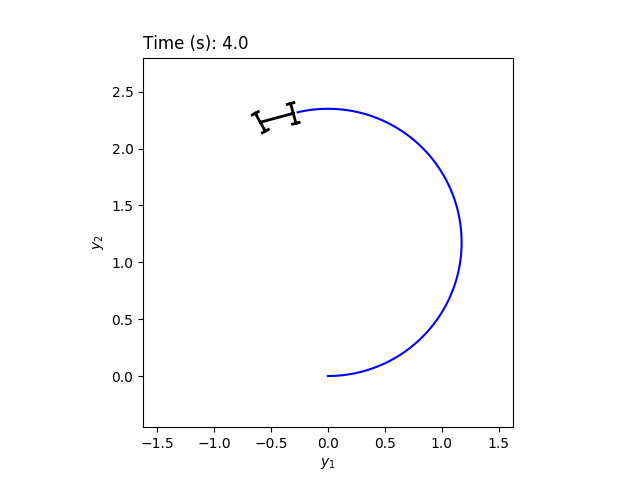
\includegraphics[width=0.7\textwidth]{img/animation}
	\caption{Car animation}
	\label{fig:animation}
\end{figure}


\newpage
\section{Simulation with SciPy's new \emph{solve\_ivp} module and the \emph{lambda} function}
\footnote{corresponding file: \emph{car-like\_mobile\_robot\_lambda.py}}
In addition to the solution in \autoref{sec:simulation} using \emph{odeint}, SciPy's integrate package contains some newer solver classes. To use the general \emph{solve\_ivp} class, we need to import the new package.
\begin{lstlisting}
from scipy.integrate import solve_ivp
\end{lstlisting}
Then we have to switch the arguments of our \emph{ode}-function, because in \emph{solve\_ivp} the desired order of function arguments in the ODE is different. We therefore replace
\begin{lstlisting}
def ode(x, t, prmtrs):
\end{lstlisting}
with 
\begin{lstlisting}
def ode(t, x, prmtrs):
\end{lstlisting}
Now we can call the solver.
\begin{lstlisting}
sol = solve_ivp(lambda t, x: ode(t, x, prmtrs), 
               (t0, tend), x0, method='RK45',t_eval=tt)
\end{lstlisting}
The arguments of \emph{solve\_ivp} differ from \emph{odeint}. The ODE must have the form $f(t,x)$. In order to use \emph{ode(t, x, prmtrs)}, which takes 3 arguments, we need to use a \emph{lambda} function. This way we encapsulate the ODE in an anonymous function, that has just $(t, x)$ as arguments and can be evaluated by \emph{solve\_ivp}.\footnote{the lambda function corresponds to @ in \emph{MATLAB}} After the ODE is passed the solver takes the following arguments: a tuple $(t0, tend)$ which defines the simulation interval, the initial value $x0$. Additionally we pass the optional arguments \emph{method}, in this case a Runge-Kutta method and \emph{t\_eval}, which defines the values at which the solution should be sampled. 
The return value \emph{sol} is an \emph{OdeResult} object. To extract the simulated state trajectory, we execute:
\begin{lstlisting}
x_traj = sol.y.T # size=len(x)*len(tt) (.T -> transpose)
\end{lstlisting}

\newpage
\section{(Differential) flatness based tracking control}
For controlling a nonlinear system like \eqref{eq:ss_system}, linear control methods are not sufficient. We therefore use an advanced control method called (differential) flatness based tracking control, where we design a model based feedforward control and stabilize the system along a planned state trajectory.
\subsection{(Differential) flatness}
A system $\dot{\x}=f(\x,\uu)$ is called (differntially) flat, if a tuple of differential independent variables exists, from which we can derive all other system variables $\z=(\x,\uu)$, without solving an ODE. Such a tuple is called a flat output $\y=h(\x)$. The flat output has $m = s-q$ components, where $s$ is the number of system variables and $q$ is the number of equations. In system \eqref{eq:syseq}, we have 5 system variables $(y_1,y_2, \theta,v, \phi) $ and 3 equations, a flat output must therefore have 2 components. A flat output is $\y=(y_1,y_2)$. We now want to show, that a function $\z = \mathbf{\psi}(\y,\dot{\y},...,\y^{(\alpha)})$ for $\y=(y_1,y_2)$ exists.

Recapture system \eqref{eq:syseq} from \autoref{sec:model}:
\setcounter{equation}{0}
\begin{subequations}
\label{eq:1}
\begin{align}
\dot{y}_1&=v \cos (\theta) \label{eq:1a}\\
\dot{y}_2&=v \sin (\theta) \label{eq:1b}\\
\tan(\phi) &= \frac{l\dot{\theta}}{v} \label{eq:1c}
\end{align}
\end{subequations}
\setcounter{equation}{2}
Dividing \eqref{eq:1b} by \eqref{eq:1a} leads to:
\begin{subequations}
\begin{align}
\frac{\dot{y}_2}{\dot{y}_1} &=\tan(\theta) \label{eq:3a}\\
\Leftrightarrow  \theta &= \arctan\left(\frac{\dot{y}_2}{\dot{y}_1}\right) \label{eq:3b}
\end{align}
\end{subequations}
The velocity $v$ can be derived from the time derivative of the position vector $\y$.
\begin{align}
\label{eq:4}
v =\left| \mathbf{v} \right| = \left| \dot{\y} \right| = \sqrt{\dot{y}_1^2+\dot{y}_2^2}
\end{align}
We take the derivative of \eqref{eq:3b} and \eqref{eq:4} insert the result in \eqref{eq:1c}:
\begin{subequations}
\begin{align}
\tan(\phi) &= \frac{l}{\underbrace{\sqrt{\dot{y}_1^2+\dot{y}_2^2}}_{v}} \underbrace{\frac{\ddot{y}_1 \dot{y}_2 - \dot{y}_1 \ddot{y}_2}{(\dot{y}_1^2+\dot{y}_2^2)}}_{\dot{\theta}}\label{eq:5a} \\
\Leftrightarrow \phi &= \arctan\left(l \frac{\ddot{y}_1 \dot{y}_2 - \dot{y}_1 \ddot{y}_2}{(\dot{y}_1^2+\dot{y}_2^2)^{\frac{3}{2}}} 
\right) \label{eq:5b}
\end{align}
\end{subequations}
Now we have found $\z = \mathbf{\psi}(\y,\dot{\y},...,\y^{(\alpha)})$:
\begin{align}
\begin{pmatrix} z_1 \\ z_2 \\ z_3 \\ z_4 \\ z_5 \end{pmatrix} = 
\begin{pmatrix} x_1 \\ x_2 \\ x_3 \\ u_1 \\ u_2 \end{pmatrix} = 
\begin{pmatrix} y_1 \\ y_2 \\ \theta \\v \\  \phi \end{pmatrix} =
\begin{pmatrix} y_1 \\ y_2 \\  \arctan\left(\frac{\dot{y}_2}{\dot{y}_1}\right)\\ \sqrt{\dot{y}_1^2+\dot{y}_2^2}\\ \arctan\left(l \frac{\ddot{y}_1 \dot{y}_2 - \dot{y}_1 \ddot{y}_2}{(\dot{y}_1^2+\dot{y}_2^2)^{\frac{3}{2}}} 
\right) \end{pmatrix}
\end{align}
$\y = (y_1, y_2)$ is indeed a flat output.
%\subsection{Transformation to BINF, determine control laws}
\subsection{Dynamic state feedback via exact input-output linearization}
In order to determine a control law we linearize the system by defining a new input $\mathbf{w}=(w_1,w_2)$. To do this we have to take the derivative of the flat output $\y$, until the input $\uu$ shows up explicitly. 
\begin{subequations}
\begin{align}
y_1 &= x_1 \\
y_2 &= x_2 \\
\dot{y}_1 &= \dot{x}_1 = u_1 \cos(x_3)\\
\dot{y}_2 &= \dot{x}_2 = u_1 \sin(x_3) \overset{!}{=} w_1 \label{eq:7d}\\
\ddot{y}_1 &= \frac{\d}{\d t}(u_1 \cos(x_3)) = \dot{u}_1 \cos(x_3) - \frac{1}{l}u_1^2\sin(x_3)\tan(u_2) \overset{!}{=} w_2 \label{eq:7e}
\end{align}
\end{subequations}
With a generalized state vector $\mathbf{q} = (q_1,q_2,q_3)^\textrm{T}=(y_1,\dot{y}_1,y_2)^\textrm{T}$ we now get a new linear state space model $\dot{\mathbf{q}}=g(\mathbf{q},\mathbf{w})$:
\begin{align}
\label{eq:8}
\begin{pmatrix}
\dot{q}_1 \\\dot{q}_2 \\ \dot{q}_3
\end{pmatrix}
=
\begin{pmatrix}
q_2 \\ w_2 \\ w_1
\end{pmatrix}
\end{align}
\subsubsection{Stabilizing the linearized system}
To stabilize system \eqref{eq:8}, we define a differential equation for the tracking error $\mathbf{e}=\y-\y_d$:
\begin{align}
\label{eq:9}
0 = \ddot{\mathbf{e}} + \mathbf{K}_1 \dot{\mathbf{e}}+\mathbf{K}_0 \mathbf{e}
\end{align}
We choose the matrices $\mathbf{K}_0$ and $\mathbf{K}_1$ such that the ODE is stable.
If we solve \eqref{eq:9} for $\mathbf{w}$ we get:
\begin{subequations}
\label{eq:10}
\begin{align}
w_1 &=  \dot{y}_2 =\dot{y}_{2,d} - k_{0,2}(y_2-y_{2,d}) \\
w_2 &= \ddot{y}_1 = \ddot{y}_{1,d} - k_{1,1}(\dot{y}_1-\dot{y}_{1,d})-k_{0,1}(y_1-y_{1,d})
\end{align}
\end{subequations}
\subsubsection{Control law}
To determine the control laws, we first substitute \eqref{eq:10} into \eqref{eq:7d} and solve for $u_1$. 
\begin{subequations}
\begin{align}
&u_1 = \frac{w_1}{\sin{x_3}} \\
\Leftrightarrow \quad & u_1 = \frac{\dot{y}_{2,d} - k_{0,2}(y_2-y_{2,d})}{\sin{x_3}} \\
\Leftrightarrow \quad & u_1 = \frac{\dot{y}_{2,d} - k_{0,2}(y_2-y_{2,d})}{\sin{\left(\arctan\left(\frac{\dot{y}_2}{\dot{y}_1}\right)\right)}}
\end{align}
\end{subequations}

%\begin{subequations}
%\begin{align}
%&\dot{u}_1 \cos(x_3) - \frac{1}{l}u_1^2\sin(x_3)\tan(u_2) = w_2 \\
%\Leftrightarrow \quad & \frac{1}{l}u_1^2\sin(x_3)\tan(u_2) = \dot{u}_1 \cos(x_3) - w_2  \\
%\Leftrightarrow \quad & \tan(u_2) = \frac{l}{u_1^2\sin(x_3)}\left(\dot{u}_1 \cos(x_3) - w_2 
%\right)  \\
%\Leftrightarrow \quad & u_2 = \arctan\left(\frac{l}{u_1^2\sin(x_3)}\left(\dot{u}_1 \cos(x_3) - w_2 
%\right)
%\right)
%\end{align}
%\end{subequations}

Then substitute $\mathbf{w}$ in \eqref{eq:5b}:
\begin{subequations}
\begin{align}
u_2 &= \arctan\left(l \frac{\ddot{y}_1 \dot{y}_2 - \dot{y}_1 \ddot{y}_2}{(\dot{y}_1^2+\dot{y}_2^2)^{\frac{3}{2}}} 
\right) \\
&= \arctan\left(l \frac{w_2 w_1 - \dot{y}_1 \dot{w}_1}{(\dot{y}_1^2+w_1^2)^{\frac{3}{2}}} 
\right) 
\end{align}
\end{subequations}
The derivative of $w_1$ appears in the feedback law. We therefore have to derive the equation for it:
\begin{subequations}
\begin{align}
\dot{w}_1 = \ddot{y}_2 = \frac{\d w_1}{\d t} &= \frac{\d}{\d t}(\dot{y}_{2,d} - k_{0,2}(y_2-y_{2,d})) \\
&=\ddot{y}_{2,d} - k_{0,2}(\underbrace{\dot{y}_2}_{=w_1}-\dot{y}_{2,d}) \\
&=\ddot{y}_{2,d} - k_{0,2}(\dot{y}_{2,d} - k_{0,2}(y_2-y_{2,d})-\dot{y}_{2,d}) \\
\Leftrightarrow \quad \dot{w}_1&=\ddot{y}_{2,d} - k_{0,2}^2(y_2-y_{2,d})
\end{align}
\end{subequations}
\subsection{Calculating a reference trajectory (path planner)}
Now that we have defined the control law we need to develop a path planner, that calculates a feasible trajectory of the flat output and its derivitives (to the second order) for a given state transition.

\centering{\textcolor{red}{figure: showing a state transition}}

\subsection{Implementation of the controller in \py}
\centering{\textcolor{red}{work in progress}}

%\subsection{Plotresults}
\end{document}
